\documentclass[11pt,letterpaper]{article}
\usepackage[T1]{fontenc}
\usepackage[utf8]{inputenc}
\usepackage{lmodern,amsmath,amssymb,amsthm,mathtools}
\usepackage[margin=1in]{geometry}
\usepackage{microtype,booktabs,array,longtable,enumitem,xcolor,graphicx,needspace}
\usepackage{fancyhdr,listings}
\usepackage{tikz}
\usetikzlibrary{arrows.meta,positioning}
\definecolor{ink}{RGB}{24,47,70}
\definecolor{accent}{RGB}{0,103,113}
\usepackage[colorlinks=true,linkcolor=ink,citecolor=accent,urlcolor=accent,breaklinks]{hyperref}
\usepackage[nameinlink,noabbrev]{cleveref}
\makeatletter
\renewcommand*\l@subsection{\@dottedtocline{2}{1.5em}{3.2em}}
\makeatother
\hypersetup{pdftitle={Exact Long-Twist Recurrences and Streamed Homology for Unknot Recognition},
pdfauthor={Research continuation prepared for the ProveIt project},
pdfsubject={Finite-threshold homology, binary braid inputs, rigorous resource bounds, and a research programme toward quasi-polynomial recognition}}
\setlength{\headheight}{14pt}
\pagestyle{fancy}\fancyhf{}
\fancyhead[L]{\small ProveIt / Unknot Recognition}
\fancyhead[R]{\small Exact recurrences and streamed homology}
\fancyfoot[C]{\thepage}
\setlength{\parskip}{4pt}
\setlength{\parindent}{1.1em}
\setlist{itemsep=3pt,topsep=5pt,leftmargin=1.7em}
\newtheorem{theorem}{Theorem}[section]
\newtheorem{lemma}[theorem]{Lemma}
\newtheorem{proposition}[theorem]{Proposition}
\newtheorem{corollary}[theorem]{Corollary}
\theoremstyle{definition}
\newtheorem{definition}[theorem]{Definition}
\newtheorem{remark}[theorem]{Remark}
\newtheorem{question}[theorem]{Research question}
\newcommand{\F}{\mathbb F_2}
\newcommand{\Z}{\mathbb Z}
\newcommand{\N}{\mathcal N}
\newcommand{\Kh}{\operatorname{Kh}}
\newcommand{\rKh}{\widetilde{\operatorname{Kh}}}
\newcommand{\rank}{\operatorname{rank}}
\newcommand{\poly}{\operatorname{poly}}
\newcommand{\supp}{\operatorname{supp}}
\newcommand{\code}[1]{\texttt{\detokenize{#1}}}
\lstset{basicstyle=\small\ttfamily,breaklines=true,columns=fullflexible,
keepspaces=true,frame=single,rulecolor=\color{black!20},
xleftmargin=0.4em,xrightmargin=0.4em,showstringspaces=false}
\begin{document}
\hypersetup{pageanchor=false}
\begin{titlepage}
\thispagestyle{empty}
\vspace*{0.15in}
\noindent{\large\scshape ProveIt research continuation}\par
\vspace{0.32in}
\noindent{\Huge\bfseries\color{ink} Exact Long-Twist\\[5pt]
Recurrences and\\[5pt] Streamed Homology}\par
\vspace{0.22in}
\noindent{\Large for Unknot Recognition}\par
\vspace{0.23in}
\noindent Finite thresholds, compressed braid inputs, measured implementation
tradeoffs, and the remaining quasi-polynomial problem\par
\vspace{0.22in}
\noindent Prepared for Vladimir Reshetnikov's ProveIt project\\
8 October 2026\par
\vspace{0.18in}\hrule\vspace{0.12in}
\begin{abstract}
We continue the integrated twist-compression and component-algebra work in
ProveIt at revision \code{ea2abcb115aaa58f0b193ce1e045c2def983e1e6}.
For a signed braid with one variable run \(\sigma_i^{\varepsilon m}\), freeze
the other runs and let their total crossing count be \(W\). We prove that
one reduced characteristic-two Khovanov computation at \(m_0=W+2\) determines
the entire homological-degree profile for every \(m\ge m_0\).
Two fixed finite boundary pieces are separated by a constant-rank interval;
the exact rank is
\[
R(m)=R(m_0)+(m-m_0)\eta,\qquad
\eta=\dim_{\F}\rKh(J_E;\F)>0,
\]
where \(J_E\) is the closure with the selected run replaced by its turnback
smoothing. The proof uses the repeated differential \(D_E+X_p+X_q\),
not just repeated chain dimensions. Jaeger's weighted-dot theorem identifies
the slope. A compact output makes the exponent dependence polynomial in
its bit length for fixed context.

We implement the recurrence, a degree-streamed exact backend with bounded
state and map caches, and direct structural certificates for run-encoded
braids. Paired experiments show substantial standalone homology gains from
the recurrence and a measurable time--space tradeoff from streaming.
Independent crossing-cube comparisons check both signed gradings and the
full homological profiles. We also prove that a proposed definite-signature
shortcut is dominated by the existing Rasmussen interval, and that this
interval already decides every knot in the recurrence's dominant-run range.
Thus the new exact-homology result does not enlarge that decision class.
The work gives precise restricted-input bounds and an implementable research
programme; it does not establish unrestricted quasi-polynomial recognition.
\end{abstract}
\vfill
\noindent\small Deliverable: a reproducible article, additive implementation,
regression tests, independent audits, raw measurements, and a patch against
the pinned baseline. Mathematical proofs and executable checks are
distinguished throughout.
\end{titlepage}
\hypersetup{pageanchor=true}
\pagenumbering{roman}
\tableofcontents
\clearpage
\pagenumbering{arabic}
\section{Conclusions, baseline, and research scope}\label{sec:scope}

The strongest new mathematical step in this continuation is an exact
finite-threshold recurrence for one long twist region. The existing
support-counting formula says that the chain dimension grows affinely in a
selected exponent. We pass from that statement about the number of
generators to a statement about the differential and hence the actual
homology. This distinction matters: a repeated vector space can carry
different differentials, and chain-size growth alone does not determine
homology growth.

The implementation work has two complementary purposes. The recurrence
avoids constructing an arbitrarily long repeated part. The streamed backend
reduces retained storage when the finite complex still needs to be evaluated.
Direct braid-source structural bounds avoid expanding a binary exponent
merely to rediscover a certificate already available from elementary counts.
Each change has an explicit interface and an independently stated scope.

\subsection{What is already in ProveIt}

The baseline is the repository's main revision
\code{ea2abcb115aaa58f0b193ce1e045c2def983e1e6}, retrieved on 8 October 2026.
The immediately relevant integrated work comprises report 10 on structural
and algebraic improvements, report 11 on twist compression, report 12 on
component algebra, and their synthesis updates~\cite{repo}.
The complete \code{fast/} Python source, tests, examples, and build metadata
at this revision accompany the package as a reference snapshot.

The current recognizer already has much more than a naive crossing cube.
Its pipeline contains checked diagram construction, braid certificates
including the at-most-three-strand endpoint, signed Seifert-graph criteria,
diagram simplification, visible connected-sum and interlacement
factorization, modular Alexander and Jones obstructions, and exact
Khovanov scanning. Optional paths provide a twist macro backend and
component-algebra contractions. Existing scan machinery includes local
gluing, unit cancellation, bit-packed linear algebra, and choices of scan
order. Those features are baseline capabilities, not contributions of this
continuation.

In particular, report 11 explicitly proposed degree-streamed rank
computation and required the state generator and map caches to be included
in its memory analysis. We implement that proposal rather than presenting
the rank identity underlying it as a new mathematical discovery.
Report 11 also established, for supplied signed runs with lengths \(m_j\),
the support polynomial
\begin{equation}\label{eq:support}
\N=\sum_{S\subseteq[t]}2^{c(S)-1}\prod_{j\in S}m_j
\end{equation}
and a restricted-family complexity bound
\begin{equation}\label{eq:prior-bound}
\poly(n)\,2^{O(t\log(2+n/t))},\qquad n=\sum_jm_j.
\end{equation}
Here \(c(S)\) is the number of circles after choosing the turnback exactly
in the boxes in \(S\). The run count \(t\) is the count in the supplied
presentation. It is not a proven small invariant of every knot.

\begin{center}
\small
\begin{tabular}{p{0.43\linewidth}p{0.48\linewidth}}
\toprule
Result or capability & Status in this continuation\\
\midrule
Two-strand twist normal form; Khovanov unknot detector &
Established literature, used with explicit attribution.\\
Support polynomial and \(t=O(\log n)\) bound &
Already integrated in the pinned ProveIt baseline.\\
One-reference signed homology recurrence and slope extraction &
Proved here as a continuation of that model; implemented.\\
Slope as reduced homology of the turnback closure &
Proved using established dot-sliding and local contraction machinery.\\
Degree-streamed ranks, bounded caches, early lower bound &
Implemented with exact accounting and regression checks.\\
Structural certificates on binary run input &
An encoding improvement to existing sufficient conditions.\\
New signature packing decision class &
None: the proposed bound is proved dominated.\\
Unrestricted quasi-polynomial recognition &
Not established by this work.\\
\bottomrule
\end{tabular}
\end{center}

\subsection{Current literature and the asymptotic target}

The mathematical local input is Bar--Natan's tangle category and
cancellation calculus~\cite{bn05,bn07}, with integer-twist complexes
described explicitly by Thompson~\cite{thompson}. The rank-one decision
criterion is due to Kronheimer and Mrowka~\cite{km}.
Twist stabilization and compact tangle descriptions have substantial
precedent, including the immersed-curve framework of Kotelskiy, Watson,
and Zibrowius~\cite{kwz}. The finite threshold and one-reference extraction
below should be assessed as a precise, executable continuation of the
repository's model. We make no general priority claim for stability under
twisting.

Kelom\"aki and Sch\"utz's 2026 preprint supplies an especially useful
boundary for complexity arguments: their Theorem 1.2 gives exponential
scanning behavior on certain three-strand braid families, whereas their
Theorem 1.3 gives a specialized polynomial-time computation for all
three-strand braids~\cite{ks26}. A bounded number of boundary matching
types therefore cannot, by itself, bound the number of algebraic summands.
The specialized theorem also prevents a misleading benchmark claim:
three-strand examples are useful algebraic checks, but do not demonstrate
new difficult instances for the integrated recognizer.

The hierarchy route must be described separately. Lackenby's July 2026
preprint develops incompressible surfaces, boundary patterns, and unknot
recognition. Section 9 bounds iterations while explicitly leaving costs
of steps insufficiently specified for a complete runtime estimate;
Proposition 9.1 gives \(L(g+1)^L\) iterations in its hierarchy and pattern
parameters~\cite{lackenby26}. Other results provide compact surface
certificates and algorithms polynomial in handle data and logarithmic
normal weight. Those facts support a serious alternative research
programme, but they do not supply the missing cost theorem for the present
Khovanov implementation. Certificate existence, certificate verification,
certificate search, and repeated compressed operations remain different
tasks.

We also inspected the user-suggested \code{openai/math} catalogue and
repository guidance~\cite{openaimath}. Its manuscripts have varying
verification status. No theorem from that collection is needed for the
proofs here; a superficially similar quasi-polynomial result in a different
subject would not remove the particular representation and rank barriers
identified below. The useful methodological lesson is to keep dependencies,
proof status, and machine-checkable artifacts explicit.

\subsection{Four sizes that must be kept distinct}

Let
\begin{equation}\label{eq:input}
\beta=\sigma_{i_1}^{e_1}\cdots\sigma_{i_t}^{e_t},\qquad
1\le i_j<b,\quad e_j\in\Z\setminus\{0\}.
\end{equation}
Put \(m_j=|e_j|\), \(n=\sum_jm_j\), and define the encoded input size,
up to a fixed choice of delimiters, by
\begin{equation}\label{eq:encoded}
\lambda=1+\lceil\log_2(b+1)\rceil+
\sum_{j=1}^t\bigl(1+\lceil\log_2(b+1)\rceil+
                         \lceil\log_2(m_j+1)\rceil\bigr).
\end{equation}
An expanded braid word has length \(n\). A run-encoded braid can have
\(n\) exponential in \(\lambda\). A planar diagram normally presents its
crossings explicitly and therefore has a different input model.

There are also the number \(S=\prod_j(m_j+1)\) of macro states, the total
reduced chain dimension \(\N\), and the bit length of the requested output.
A scalar formula for \(\N\) does not compute a differential rank. A
compact formula for a homological profile is a different output from an
explicit dictionary containing each degree. We charge for the chosen
representation throughout.

The closure of a braid is a knot exactly when its strand permutation is a
single cycle. A run contributes the adjacent transposition only when its
exponent is odd. Thus original component count is computable without
expanding any run. For a one-component \(b\)-braid every generator index
\(1,\ldots,b-1\) occurs; omitting index \(i\) separates the first \(i\)
strands from the others. This simple fact gives \(b-1\le t\) and will also
control the reference size in the dominant-run theorem.

\subsection{The characteristic-two exact endpoint}

For a knot \(K\), the endpoint used here is
\begin{equation}\label{eq:detector}
K\text{ is the unknot}\quad\Longleftrightarrow\quad
\dim_{\F}\rKh(K;\F)=1.
\end{equation}
The implication from rank one follows from the rational rank-one detector
of Kronheimer--Mrowka and the universal coefficient theorem: characteristic
two dimension is at least the rational dimension, and reduced homology is
nonzero. The unknot has one reduced generator over either field.
All calculations retain a fixed reduction point. For links we compute
reduced homology at that point, but do not apply a knot-only decision
criterion to them.

Resource exhaustion has a precise meaning. A mathematical exact algorithm
without fixed caps terminates on finite inputs. Its resource-bounded
implementation can return \code{UNKNOWN}. Such a result is neither
evidence of knottedness nor evidence of triviality. The same distinction
applies when a computation has established only a lower bound on the
homology dimension.

\section{The local complex and its global counts}\label{sec:local}

We use \(A=\F[X]/(X^2)\), with
\[
\Delta(1)=1\otimes X+X\otimes1,\qquad \Delta(X)=X\otimes X.
\]
A resolution with \(c\) circles has reduced space of dimension
\(2^{c-1}\): the circle containing the fixed mark carries \(X\), and each
other circle carries \(1\) or \(X\).
Let \(I\) denote the identity two-strand matching and \(E\) the matching
joining the two top ends and joining the two bottom ends. Names such as
cap and cup depend on drawing orientation; the chosen arcs are always
identified as the top and bottom arcs of \(E\).

\begin{proposition}[Established local normal form]\label{prop:normal}
After forgetting quantum grading, a positive run of length \(m\) is
represented by
\[
I\xrightarrow{s}E\xrightarrow{L}E\xrightarrow{L}\cdots
\xrightarrow{L}E,\qquad L=X_{\rm top}+X_{\rm bottom},
\]
in degrees \(0,1,\ldots,m\). A negative run is represented by its dual
complex in degrees \(-m,\ldots,-1,0\), with \(I\) in degree zero, the final
saddle into \(I\), and the same internal dot sum.
The replacement is valid inside any fixed exterior tangle.
\end{proposition}

\begin{proof}
This is the characteristic-two, quantum-forgotten specialization of the
integer-twist normal form~\cite[Proposition 4.1]{thompson}. Tensoring with
one additional crossing gives an \(E\)-circle summand. Delooping that circle
and cancelling an invertible saddle block gives the next zig-zag term.
The local contraction formula is the categorical Schur complement of
Bar--Natan~\cite{bn07}. Over the integers the internal maps have alternating
signs; the dot sum and difference agree over \(\F\). Mirroring reverses
degrees and dualizes saddles. These operations are relative to the
boundary, which justifies the stated exterior compatibility.
\end{proof}

In the tensor product of run complexes, a state has coordinates
\(0\le k_j\le m_j\). Its degree is \(\sum_j\operatorname{sign}(e_j)k_j\).
Its geometry depends only on the support \(\{j:k_j\ne0\}\), while its
differentials also distinguish the first saddle from internal dot maps.
For a fixed support \(S\), the number of coordinate choices is
\(\prod_{j\in S}m_j\). This proves \eqref{eq:support}.
The independence of geometry from the nonzero coordinate is also the
key to the stronger homology result below.

For later accounting define
\begin{equation}\label{eq:layers}
d_h=\dim C^h,\qquad r_h=\rank(\partial_h:C^h\longrightarrow C^{h+1}),
\qquad \N=\sum_h d_h.
\end{equation}
The exact formula
\begin{equation}\label{eq:betti}
\beta_h=\dim H^h=d_h-r_{h-1}-r_h
\end{equation}
uses both incident boundary ranks. Computing only chain dimensions, only
one boundary rank, or a rank bound in the wrong direction cannot justify
an exact Betti number.

Two convenient coarse quantities are
\[
Q=\sum_h d_hd_{h+1},\qquad
T_{\rm elim}=
O\!\left(\N+\sum_h d_h d_{h+1}\min(d_h,d_{h+1})\right)
\]
for elimination once the actual columns are supplied. Generating states
and local maps is a separate cost; it is included explicitly in the
algorithm bounds below. The \(\N\) term also charges for visiting zero
columns and end degrees.
\(Q\) is a dense bit envelope, not a count of actual nonzero entries.
The displayed elimination term is a conservative bit-operation bound for
ordinary characteristic-two Gaussian elimination. It is enough for
asymptotic upper bounds; it is not a claim that Python attains an optimal
matrix multiplication exponent.

\section{An exact finite-threshold recurrence}\label{sec:recurrence}

Select one run position in \eqref{eq:input}, and keep its generator,
its sign \(\varepsilon\), and every other run fixed. Only its absolute
exponent \(m\ge1\) varies. Define
\begin{equation}\label{eq:context-span}
a=-\sum_{\substack{j\ne *\\e_j<0}}|e_j|,\qquad
c=\sum_{\substack{j\ne *\\e_j>0}}|e_j|,\qquad
W=c-a,\qquad m_0=W+2.
\end{equation}
The letter \(c\) here is a degree endpoint, not a circle count or the
number \(b\) of braid strands. Empty sums are zero.

\subsection{The fixed context and its repeated differential}

For each context degree \(q\), let \(I^q\) be the direct sum of reduced
resolution spaces when the distinguished box contains \(I\), and let
\(E^q\) be the corresponding sum with \(E\) in that box. Both vanish
outside \([a,c]\). All other run differentials define \(D_I\) and \(D_E\).
The chosen saddle maps between the two sectors in the direction determined
by \(\varepsilon\). Write
\begin{equation}\label{eq:context-space}
V=\bigoplus_{q=a}^{c}E^q,\quad M=\dim V,\quad
L=X_p+X_q,\quad F=D_E+L,\quad
r=\rank F,\quad \eta=M-2r.
\end{equation}
In \(X_p+X_q\), the subscripts designate the two exterior arc points,
independently of the context degree index.
The operator \(D_E\) raises context degree, while \(L\) preserves it.
Consequently \(F\) is initially an endomorphism of the \emph{ungraded}
space \(V\).

\begin{lemma}\label{lem:square-zero}
The operator \(F\) satisfies \(F^2=0\), and
\(\eta=\dim H(V,F)\ge0\).
\end{lemma}

\begin{proof}
The context is a chain complex, so \(D_E^2=0\). Each dot squares to zero,
and distinct dots commute; hence \(L^2=0\) in characteristic two.
Multiplication and comultiplication commute with a dot on an unchanged
arc:
\[
m(X\otimes1)=Xm=m(1\otimes X),\qquad
(X\otimes1)\Delta=\Delta X=(1\otimes X)\Delta.
\]
These are direct identities in \(A\), including on the marked-\(X\)
subcomplex. Thus \(D_EL=LD_E\), and the mixed terms in \(F^2\) cancel.
Finally, \(\operatorname{im}F\subseteq\ker F\); rank--nullity gives
\(\dim\ker F-\dim\operatorname{im}F=M-2r\).
\end{proof}

The identity \(F^2=0\) is stronger than a numerical observation about
consecutive ranks. Its use is specific to the characteristic-two normal
form just specified. An integral or odd-characteristic version needs its
own signs, gradings, and differential analysis.

\subsection{Where complete context groups occur}

For a positive distinguished run, the summand \(E^q\) lies in total degree
\(h=q+k\), with \(1\le k\le m\). Therefore
\begin{equation}\label{eq:positive-central}
C_m^h=V\quad\text{throughout}\quad c+1\le h\le a+m.
\end{equation}
Indeed, these inequalities are exactly the conditions that every
\(q\in[a,c]\) has \(1\le h-q\le m\). The \(I\) sector is absent in
this interval because \(h>c\).
Between two adjacent groups satisfying \eqref{eq:positive-central},
the other-run maps give \(D_E\) and the distinguished internal maps give
\(L\). Under the canonical identification by context state and circle
label, the differential is exactly \(F\).

For a negative distinguished run, \(h=q-k\) instead. Complete groups and
their internal differentials occur in
\begin{equation}\label{eq:negative-central}
c-m\le h\le a-1,\qquad
\partial_h=F\quad(c-m\le h\le a-2).
\end{equation}
Here the \(I\) sector is absent because \(h<a\).
These descriptions keep the mixed signs in the context; no assumption
that the braid is positive, alternating, or homogeneous has entered.

At \(m=m_0\), there are exactly two consecutive complete groups. In the
positive case they are in degrees \(c+1,c+2\); in the negative case they
are in degrees \(a-2,a-1\). The single map between them is \(F\).
The two-group threshold is deliberate. One complete group alone does not
expose a complete central differential, and its Betti number can still
depend on both boundary regions.

\subsection{The two signed profile formulas}

Let
\[
P_m(z)=\sum_h\dim_{\F}H^h(C_m)\,z^h
\]
be the reduced homological Laurent polynomial, with quantum grading
forgotten and the macro grading fixed as in \cref{prop:normal}.

\begin{theorem}[One-reference recurrence]\label{thm:recurrence}
Set \(m_0=W+2\), \(\delta=m-m_0\), and compute \(P_{m_0}\).
For a positive distinguished run, split it into
\[
P_{\rm low}=\sum_{h\le c+1}\beta_h(m_0)z^h,\qquad
P_{\rm high}=\sum_{h\ge c+2}\beta_h(m_0)z^h.
\]
Then for every \(m\ge m_0\),
\begin{equation}\label{eq:positive-profile}
\boxed{\displaystyle
P_m(z)=P_{\rm low}(z)+z^\delta P_{\rm high}(z)
       +\eta\sum_{h=c+2}^{a+m-1}z^h.}
\end{equation}
For a negative distinguished run, put
\[
Q_{\rm low}=\sum_{h\le a-2}\beta_h(m_0)z^h,\qquad
Q_{\rm high}=\sum_{h\ge a-1}\beta_h(m_0)z^h.
\]
Then
\begin{equation}\label{eq:negative-profile}
\boxed{\displaystyle
P_m(z)=z^{-\delta}Q_{\rm low}(z)+Q_{\rm high}(z)
       +\eta\sum_{h=c-m+1}^{a-2}z^h.}
\end{equation}
An interval sum with lower endpoint above its upper endpoint is empty.
In either case the total reduced rank obeys
\begin{equation}\label{eq:rank-recurrence}
R(m)=R(m_0)+(m-m_0)\eta.
\end{equation}
The statement permits links and any fixed exterior reduction point.
\end{theorem}

\begin{proof}
First suppose the distinguished run is positive. Near the lower end,
the condition \(k\le m\) is inactive once \(m\ge m_0\).
Every chain group in degrees at most \(c+1\), its incoming map, and its
outgoing map are therefore the same as at \(m_0\).
At the top, writing \(k'=k-\delta\) identifies all groups in degrees at
least \(c+2+\delta\), together with both incident maps, with the reference
upper region translated by \(\delta\). This can also be read directly
from \(1\le h-q\le m\): near that end the lower bound is inactive.
The saddle into the first \(E\) sector remains in the fixed lower region.

The degrees strictly between these two regions are
\(c+2,\ldots,a+m-1\). Each has chain space \(V\), incoming map \(F\),
and outgoing map \(F\). Its Betti number is \(M-r-r=\eta\).
There are \(m-m_0\) such degrees. Applying \eqref{eq:betti} in the fixed
and translated boundary regions proves \eqref{eq:positive-profile}.

For a negative run, use \(1\le q-h\le m\). The lower region now
translates downward by \(\delta\), while the upper region, including
the saddle into \(I\), remains fixed. Its separating complete groups
are \eqref{eq:negative-central}. The inserted degrees are precisely
\(c-m+1,\ldots,a-2\), again with both maps \(F\).
This proves \eqref{eq:negative-profile}. Evaluating at \(z=1\) gives
\eqref{eq:rank-recurrence}.
\end{proof}

This proof identifies the boundary maps as well as the central chain
groups. Without that step, shifting observed Betti numbers would be an
unjustified extrapolation. It also explains why the reference can be a
link of different component count: the argument is a statement about
marked complexes, not an isotopy between the original and reference
closures.

\begin{corollary}[Extraction from existing output]\label{cor:extraction}
The ordinary macro output at \(m_0\), which reports chain dimensions
and boundary ranks, determines \(\eta\) without a second homology
computation. Use
\[
h_*=\begin{cases}c+1&\varepsilon=+1,\\a-2&\varepsilon=-1,\end{cases}
\qquad
M=d_{h_*}=d_{h_*+1},\quad r=r_{h_*},\quad \eta=M-2r.
\]
\end{corollary}

The threshold Betti numbers at \(h_*\) and \(h_*+1\) need not equal
\(\eta\). They are boundary-region values. This distinction is covered
by tests comparing the extracted slope with the newly interior degree
at \(m_0+1\), in addition to tests of total ranks.

\subsection{Chain savings and a concrete family}

Let \(A_0=\sum_q\dim I^q\), \(B_0=\sum_q\dim E^q=M\).
The original and reference chain dimensions are exactly
\begin{equation}\label{eq:chain-saving}
\N(m)=A_0+mB_0,\qquad
\N_0=A_0+(W+2)B_0.
\end{equation}
The coefficient \(B_0\) counts repeated chain generators.
The coefficient \(\eta=B_0-2\rank F\) counts repeated homology.
They are usually different.

For example, take
\[
\beta_m=\sigma_1^m\sigma_2^{-1}\sigma_1\sigma_2^{-1}
\quad\text{on three strands},\qquad m\ge5.
\]
Here \((a,c,W,m_0)=(-2,1,3,5)\). The reference computation gives
\(\N_0=93\), \(B_0=15\), \(r=6\), and \(\eta=3\), while
\(\N(m)=15m+18\) and \(R(m)=3m+2\).
The result applies to every integer \(m\ge5\), including link parities;
odd \(m\) gives a knot. The figure included with the experiments plots
the full degree profile and its translated upper boundary.
This is a useful exact test family, not a hard recognition family:
the baseline already has structural and three-strand certificates.

\section{The slope is the homology of the smoothing closure}
\label{slope-section}

The finite-threshold recurrence identifies its slope as the homology dimension
of a repeated differential. We now identify that number topologically. This
also proves that the repeated part cannot disappear. All vector spaces in this
section are over $\F$, and the reduction point is fixed on a closing arc
outside the run boxes. Let
\[
 V=\bigoplus_q E^q,\qquad F=D_E+L,\qquad
 L=X_p+X_q,\qquad
 \eta=\dim V-2\operatorname{rank}F,
\]
where $p$ and $q$ lie on the cap and cup of the distinguished $E$ smoothing.
Here $D_E$ is the context differential. The notation $X_p$ denotes the
usual dot action, namely multiplication by $X$ on the resolution circle
containing $p$. Let $J_E$ be the actual link diagram obtained by replacing
the entire distinguished run by that smoothing. The identification below
concerns total homology dimension; it does not identify the original
homological grading on the summands of $V$ with a grading on $H(V,F)$.

\subsection{The two dots lie on one actual component}

\begin{lemma}\label{slope-cap-cup}
The cap and cup of the distinguished smoothing belong to the same component
of $J_E$, for every choice of the other signed braid runs.
\end{lemma}

\begin{proof}
Remove the interior of the smoothing box and retain the four cut ends. The
outside diagram consists of closed components and two open paths. The braid
orientation implies that each open path joins a top cut end to a bottom
cut end: two ends of the same kind cannot be the ends of a coherently
oriented outside path. Consequently the outside matching of these four ends is
one of the two top-to-bottom matchings. Joining the two top ends by the cap
and the two bottom ends by the cup produces a single closed component in
either case. This component contains both smoothing arcs. The argument
concerns the actual strands, with crossings retained. In a complete
resolution the two arcs can lie on different circles, so it would be
incorrect to set $L=0$ state by state.
\end{proof}

\subsection{The characteristic-two weight slide}

Jaeger's weighted-dot construction proves that, in characteristic two,
relocating markings while preserving their total weight on every actual
component preserves the twisted complex~\cite[Theorem~3.1]{jaeger}. We give
the local algebra needed here, including its compatibility with reduction.
It supplies an explicit change of basis, a stronger statement than merely
saying that two dot actions induce the same homology map.

\begin{lemma}\label{slope-slide}
Let $(K,d)$ be the ordinary crossing-cube complex of a link, with its
gradings forgotten. Suppose $p,p'$ are successive points of one actual
strand, separated by one crossing. If $W$ is any sum of fixed-arc dot
actions and $W'=W+X_p+X_{p'}$, then $(K,d+W)$ and $(K,d+W')$ are isomorphic
as vector spaces equipped with square-zero endomorphisms. The isomorphism
preserves the reduced subcomplex at a fixed marked point.
\end{lemma}

\begin{proof}
Use the Frobenius algebra $A=\F[X]/(X^2)$, with multiplication $m$ and
comultiplication
\[
 \Delta(1)=1\otimes X+X\otimes1,\qquad
 \Delta(X)=X\otimes X.
\]
Direct evaluation on the basis gives
\begin{align}
 m\Delta&=0,&
 \Delta m&=X\otimes1+1\otimes X,\label{slope-frobenius}\\
 m(X\otimes1)&=Xm=m(1\otimes X),&
 (X\otimes1)\Delta&=\Delta X=(1\otimes X)\Delta.
 \label{slope-naturality}
\end{align}
The notation on the right of the first line means the corresponding
endomorphism of $A\otimes A$.
Dot operators commute and square to zero; they also commute with the cube
differential by \eqref{slope-naturality}. Thus $(d+W)^2=0$ for every $W$
in the statement.

Let $H$ be the reverse saddle at the selected crossing: it changes its cube
coordinate from $1$ to $0$, uses the saddle opposite to the ordinary
differential, and is zero in the other direction. Thus $H^2=0$.
Saddles at other cube coordinates commute with $H$; their two occurrences
in $dH+Hd$ cancel in characteristic two. At the selected crossing,
\eqref{slope-frobenius} gives
\[
 dH+Hd=X_p+X_{p'}=:T.
\]
Moreover $TH=0$. If the reverse saddle merges, its two output dot actions
agree and sum to zero. If it splits, the assertion follows from
$(X\otimes1+1\otimes X)\Delta=0$. Equation~\eqref{slope-naturality}
shows that each fixed-arc dot commutes with $H$, including the dots
appearing in $W$. Therefore
\begin{align*}
 (d+W')(1+H)+(1+H)(d+W)
 &=dH+Hd+(W'+W)+W'H+HW\\
 &=T+T+WH+HW+TH=0.
\end{align*}
Since $(1+H)^2=1$, this proves the claimed isomorphism.

If $z$ is the reduction point, then $H$ commutes with $X_z$ by the same
local identities. Hence $1+H$ preserves $\operatorname{im}X_z$, the
subcomplex in which the marked resolution circle is labeled $X$. Its
inverse does so as well. This also covers the case where $z$ belongs to a
different component from the moving dots.
\end{proof}

Repeatedly applying the lemma moves a dot along any path in its actual
component. Two unit weights meeting at one point cancel because $1+1=0$.
By Lemma~\ref{slope-cap-cup}, the reduced cube of $J_E$ with differential
$d+X_p+X_q$ is consequently isomorphic to its ordinary reduced cube.
This argument uses a sequence of local invertible maps. A general
null-homotopy $T=dH+Hd$ would not, by itself, justify replacing $d+T$ by
$d$; the identities $H^2=0$ and $TH=0$ are what make the displayed
conjugation work.

\subsection{Compatibility with the compressed context}

The preceding argument applies initially to the crossing cube. Passing to
the run complex requires compatibility of the compression with the two
exterior dots. This follows from the local cobordism construction, but it
is useful to record exactly which homotopy identities are needed.

\begin{lemma}\label{slope-compression}
Suppose $(K,d)$ and $(V,D_E)$ are related by the local Bar--Natan
reductions in the context run boxes. Let $L_K$ and $L_V$ be the sums of the
two dot actions on the distinguished smoothing arcs. Then these reductions
induce a homotopy equivalence between $(K,d+L_K)$ and $(V,D_E+L_V)$ after
forgetting the gradings. They also preserve the fixed reduction.
\end{lemma}

\begin{proof}
Bar--Natan's tangle formalism and its delooping and cancellation operations
take place in the category of local dotted cobordisms~\cite{bn05,bn07}.
An exterior marked arc is retained throughout each such operation. Sliding
a dot along its unchanged boundary cylinder shows that every local
structural map, and every local contracting homotopy, commutes with that
dot. This remains true for linear combinations and composites, and for
the maps obtained by delooping a circle inside a context box. The two
distinguished dots and the reduction point are outside those boxes.

More explicitly, choose the resulting maps $f:K\to V$, $g:V\to K$ and
homotopies $h$ on $K$, $k$ on $V$. In addition to their ordinary chain-map
identities they satisfy
\[
 fL_K=L_Vf,\quad gL_V=L_Kg,\quad
 hL_K=L_Kh,\quad kL_V=L_Vk.
\]
Thus $f$ and $g$ are chain maps for the deformed differentials. Their
homotopy identities remain valid, because
\[
 gf-1=dh+hd=(d+L_K)h+h(d+L_K),
\]
and similarly
\[
 fg-1=D_Ek+kD_E=(D_E+L_V)k+k(D_E+L_V).
\]
The additional terms cancel in characteristic two. All maps commute with
the reduction dot, so the same identities restrict to the reduced
subcomplexes. Only finite complexes are involved; no completion or
infinite-twist limit enters this argument.
\end{proof}

\begin{theorem}[Topological slope]\label{slope-theorem}
For either sign of the distinguished braid run,
\begin{equation}\label{slope-identity}
 \boxed{\displaystyle
 \eta=\dim_{\F}\rKh(J_E;\F)>0.}
\end{equation}
The reduction point on the right is the original fixed point, and total
dimension is taken over all homological and quantum degrees.
\end{theorem}

\begin{proof}
Lemma~\ref{slope-compression} identifies $H(V,F)$ with the homology of the
reduced crossing cube deformed by the two dots. The weight-slide argument
identifies that cube with the ordinary reduced cube of $J_E$. This proves
the equality and shows that the slope is independent of the sign chosen
for the distinguished run.

For strict positivity, the graded Euler characteristic of ordinary reduced
integral Khovanov homology is the reduced Jones polynomial, up to the
standard normalization~\cite{bn05}. For a nonempty link with $\ell$
components, its value at $1$ has absolute value $2^{\ell-1}$ and is
nonzero. Thus the integral reduced homology has a nonzero free summand.
The universal coefficient theorem then gives nonzero reduced homology
over $\F$. The diagram $J_E$ is nonempty, so this applies even when it is
a link with several components.
\end{proof}

\begin{remark}\label{slope-grading}
The dot deformation combines maps of different original bidegrees.
Jaeger's formulation retains a collapsed $\delta$ grading, and forgetting
that grading is sufficient for \eqref{slope-identity}. The formula does
not recover the individual homological or quantum degrees of $\rKh(J_E)$
inside the repeated part. The homological-degree profile for the original
twisted closure follows instead from the separate identification of its
successive complete $E$ groups and both incident boundary maps. These are
distinct assertions and use different grading information.
\end{remark}

\subsection{Computational consequences and output size}

Write the context interval as $[a,c]$, let $w=c-a$, and put $m_0=w+2$.
For $m\ge m_0$, set $\delta=m-m_0$. The two signed recurrence formulas
have exactly $\delta$ inserted degrees. Combining them with
Theorem~\ref{slope-theorem} gives
\begin{equation}\label{slope-rank-growth}
 R(m)=R(m_0)+\delta\,\dim_{\F}\rKh(J_E;\F),
\end{equation}
where $R$ denotes total reduced rank for either fixed choice of sign.
Every inserted degree is nonzero. In particular, this is an exact linear
growth statement with positive integer slope, not merely an upper bound
on the possible growth.

The identity provides an independent interpretation and a possible
cross-check of the slope. The algorithm need not compute $\rKh(J_E)$
separately: one reference computation at $m_0$ already contains a central
boundary equal to $F$, so that $\eta=\dim V-2\operatorname{rank}F$.
The two reference shoulder Betti numbers need not equal $\eta$; the
boundary-rank extraction is essential. The original closure's component
count remains necessary before using the Khovanov unknot-detection
criterion~\cite{km}, because shortening an exponent can change the
permutation parity and the number of components.

There is also an unconditional output-size obstruction. An explicit list
of nonzero degree--Betti-number pairs contains at least $\delta$ entries,
and therefore requires $\Omega(\delta)$ output operations. For fixed
context and growing binary-encoded $m$, this is exponential in the bit
length of $m$. A compact profile avoids that cost by retaining the two
fixed shoulders, their degree shifts, and one constant-coefficient
interval. Its dependence on the distinguished exponent is only through
binary integers of $O(\log m)$ bits. The same is true of the extra
arithmetic needed to return \eqref{slope-rank-growth}. This observation
does not bound the cost of computing the context data as the context
grows; that cost can still be exponential. It establishes the appropriate
output representation and the precise sense in which a single large
exponent can be handled without expansion.

\subsection{Position relative to existing tangle methods}

The local twist normal form, dot calculus, and cancellation machinery are
established mathematics~\cite{bn05,bn07}. Thompson gives compact zig-zag
representatives for rational-tangle Khovanov complexes~\cite{thompson}.
Jaeger's weight-moving theorem supplies the central algebra behind the
slope identification~\cite{jaeger}. Kotelskiy, Watson, and Zibrowius give
immersed-curve descriptions of four-ended tangle invariants, gluing
theorems recovering Khovanov homology, and an interpretation of the
two-strand infinite-twist construction~\cite{kwz}. These precedents make
clear why a general priority claim for twist stability would be
inappropriate.

The contribution developed here is the explicit finite threshold, the
extraction from one reference computation, the compact exact output, and
their implementation and verification relative to the pinned ProveIt
baseline. The immersed-curve viewpoint is a plausible route for studying
several variable twist regions, but obtaining useful complexity bounds
would require control of the context representation, local systems, and
gluing calculations. The one-run theorem alone supplies no such control
and does not justify a general quasi-polynomial unknot-recognition bound.

\section{The compressed algorithm and its bit complexity}\label{sec:algorithm}

\subsection{One finite solve and a compact exact answer}

The implementation in \code{fastunknot.twist.tail} has a deliberately small
mathematical interface. It validates the run list, selects a specified run
or the largest run, and computes \([a,c]\) and \(m_0\). At or below the threshold
it uses the ordinary macro backend. Above the threshold it changes
only the selected absolute exponent to \(m_0\), computes the full reference
homology and boundary ranks, and applies \cref{thm:recurrence}.

The returned degree profile consists of a dictionary of exceptional
degree--dimension pairs and at most one interval
\[
(\ell,u,\eta),\qquad
\text{meaning }\beta_h=\eta\text{ for every integer }\ell\le h\le u.
\]
The exceptional degrees are disjoint from that interval. Endpoints are
inclusive. A single-degree query uses these two components directly.
The total rank is the sum of the point coefficients plus
\((u-\ell+1)\eta\) for each interval. An explicit expansion routine is
available, but has a caller-visible limit on the number of emitted terms.

\begin{center}
\begin{minipage}{0.94\linewidth}
\begin{lstlisting}
validate the original braid and retain its component count
choose the distinguished run, with sign epsilon and length m
compute context endpoints a, c and threshold m0 = c - a + 2
if m <= m0:
    return complete ordinary macro homology as a point profile
reference = the same signed runs with selected length m0
solve the complete reference complex
hc = c + 1 if epsilon > 0 else a - 2
M = reference.chain_dimensions[hc]
r = reference.boundary_ranks[hc]
eta = M - 2*r
shift the appropriate reference boundary region by m - m0
insert the proved constant interval, if it is nonempty
return exact rank, compact profile, original components,
       reference output and recurrence certificate
\end{lstlisting}
\end{minipage}
\end{center}

The certificate records the threshold, degree endpoints, selected position,
sign, reference dimensions, central boundary rank, slope, and finite solve.
It is a transparent computational witness. The implementation does not
claim that arbitrary certificate JSON is a formal proof of the topological
normal-form theorem. The independent audit reconstructs the recurrence
without calling the production recurrence routine.

\subsection{A precise parameterized guarantee}

\begin{theorem}[Cost in the context and exponent]\label{thm:bit-cost}
Let a fixed-context family be as in \cref{thm:recurrence}. Let \(\N_0\)
be its reference chain dimension. Its exact compact reduced homological
profile can be computed using one ordinary reference solve, with safe
time bound
\begin{equation}\label{eq:reference-time}
\poly(b,W)\,\N_0^3+\poly\bigl(W,\log(m+1),\log(\N_0+1)\bigr).
\end{equation}
The exponent-dependent part of the output has polynomial bit size in
\(W+\log(m+1)+\log(\N_0+1)\).
For original one-component closures with at least one run, this gives the
coarser uniform bound
\begin{equation}\label{eq:context-exp}
2^{O(W+1)}\,\poly(\log(m+1)).
\end{equation}
Fixed resource caps can interrupt the reference solve; in that event the
bounded implementation makes no exact-rank claim.
\end{theorem}

\begin{proof}
The reference has \(2W+2\) expanded crossings. There are at most \(W\)
other nonempty runs, so \(t\le W+1\).
Each reference state can be constructed and its local Frobenius maps
evaluated in a polynomial in \(b,W\), times the number of labels processed.
Assembling the reference differential and applying ordinary elimination
is therefore bounded by the first term of \eqref{eq:reference-time}.
This intentionally loose cubic bound suffices regardless of the practical
bitset improvements.

The reference homological support has at most \(2W+3\) possible degrees.
Splitting, shifting, and summing these entries takes polynomially many
integer operations. All reference coefficients and boundary ranks are at
most \(\N_0\), and the final rank is at most
\(\N_0+m\N_0\). Degree shifts use integers of \(O(\log(m+W+2))\)
bits. Standard integer arithmetic proves the second term and the output
claim.

For the uniform knot bound, every generator occurs in the original braid.
At most one generator index is supplied only by the selected run, so
\(b-2\le W\). A support of size \(s\) has at most \(b+s\) resolution
circles: changing one \(I\) into \(E\) changes component count by at most
one. Hence, even without the sharper first-use bound from report 11,
\[
\N_0\le 2^{b-1}\prod_j(1+2m_j^{(0)})
\le 2^{b-1}3^{\,2W+2}=2^{O(W)}.
\]
Here \(1+2u\le3^u\) for integers \(u\ge1\), and \(m_j^{(0)}\)
are the reference lengths. Substituting this into
\eqref{eq:reference-time} proves \eqref{eq:context-exp}.
The reference may be a link; the argument only uses occurrence of the
original generator indices, which shortening preserves.
\end{proof}

For fixed context the finite solve is a constant with respect to \(m\),
and the remaining bit complexity is polynomial in \(\log m\). This is
the encoding improvement over expanding all \(m+1\) local terms.
In particular \(W=O((\log n)^2)\) gives \(n^{O(\log n)}\), and
\(W=O((\log\lambda)^2)\) gives \(\lambda^{O(\log\lambda)}\).
More generally, if \(W=O((\log n)^k)\) for a fixed \(k\), then
\eqref{eq:context-exp} is a quasi-polynomial homology bound in the
expanded size \(n\). If the same relation is imposed with the encoded
size \(\lambda\), it is a quasi-polynomial bound in \(\lambda\).
These are promises on the supplied context, not theorems that arbitrary
diagrams admit such a representation.

Several comparable huge runs do not satisfy the fixed-small-context
condition. For example, if two lengths are both of order \(m\), choosing
one leaves \(W\) of order \(m\). Applying the theorem once does not remove
that dependence. Any run satisfying \(m\ge W+2\) has more than half the
total crossings, so there can be at most one. Choosing the largest run
therefore finds this regime whenever it is present. This fact is not a
multivariable compression theorem.

\subsection{What can and cannot be inferred from a shortened reference}

The original strand permutation is indispensable. A two-strand run of
length \(101\) is a knot, while its reference length \(m_0=2\) is a
two-component link. Nevertheless the marked reference homology is the
correct algebraic input to the recurrence. Using the reference component
count in a recognition wrapper would be a bug.

The original crossing counts are also indispensable for a grading adapter.
The existing macro-to-scanner conversion uses
\[
h_{\rm cube}=n_+^{\rm original}-h_{\rm macro}.
\]
Substituting the shortened positive crossing count would shift the reported
homology incorrectly. The delivered raw interface retains the macro
grading explicitly. The existing one-component characteristic-two adapter
can double reduced dimensions to obtain its unreduced output, but this
knot-specific convention should not be silently transferred to general
marked links.

The flag \code{check_d2=True} checks the actual finite reference
differential. It does not construct and multiply an enormous original
matrix. The output says which finite complex was checked. General
correctness for all larger exponents rests on the proof of the recurrence.

\section{Structural certificates directly from braid runs}\label{sec:structural}

An exact algebraic improvement is valuable even when recognition can be
settled more cheaply. The audit makes this separation particularly sharp
for the dominant-run family. We first specialize the existing structural
bounds to braid counts, then prove why a proposed signature shortcut
would add no cases.

\subsection{The signed path multigraph}

Assume the original closure is one component. Let \(p_i,n_i\) be the numbers
of positive and negative occurrences of generator \(i\). Define
\[
P=\sum_i p_i,\quad N_-=\sum_i n_i,\quad n=P+N_-,\quad e=P-N_-,
\]
\[
u_+=|\{i:p_i>0\}|,\qquad u_-=|\{i:n_i>0\}|,\qquad d=n-b+1.
\]
The \(b\) oriented Seifert disks of a braid form a path multigraph, with
all crossings of \(\sigma_i\) joining vertices \(i,i+1\). The positive
and negative subgraphs have \(b-u_+\) and \(b-u_-\) connected components,
respectively, including isolated vertices.
Specializing the Kawamura--Lobb bound and the homogeneous-diagram
criterion~\cite{lobb,abe,cromwell} gives
\begin{equation}\label{eq:braid-rasmussen}
e+b-2u_+-1\ \le s(K)\le\ e-b+2u_-+1,
\end{equation}
in the usual Artin crossing-sign convention.
The canonical surface has genus \(d/2\), and the homogeneity defect is
\begin{equation}\label{eq:mixed}
u_++u_--b+1
=|\{i:p_i>0\text{ and }n_i>0\}|.
\end{equation}
The equality follows because every generator index occurs in at least
one sign.

Thus \(d=0\) certifies the unknot. If the defect is zero, the homogeneous
diagram realizes the knot genus; positive \(d\) certifies knottedness.
An interval in \eqref{eq:braid-rasmussen} excluding zero also certifies
knottedness. An interval containing zero alone does not certify triviality,
even if it consists of the single value zero.

\begin{proposition}[Encoded structural evaluation]\label{prop:rle}
All these quantities and the original one-component condition can be
computed in polynomial time in the run-encoded input size \(\lambda\),
without expanding exponents.
\end{proposition}

\begin{proof}
Accumulate signed occurrence counts and exponent sums using integer
arithmetic. Apply the adjacent transposition for each odd exponent, keeping
only touched positions in a sparse permutation. A position not touched is
fixed; add those fixed cycles to the cycles in the sparse permutation.
If some generator index is absent, reject the knot-only interface without
allocating an array of length \(b\).
Otherwise, for a knot candidate \(b-1\le t\), so all count and cycle
structures have polynomial size in \(\lambda\).
The displayed formulas then require only additions, comparisons, and
small-integer multiplications on numbers of \(O(\lambda)\) bits.
\end{proof}

The module \code{braid_profile.py} implements this specialization.
One repository sign convention needs explicit documentation.
For inputs built by \code{Diagram.from_braid}, the production Seifert
evaluator assigns the opposite sign to the usual positive Artin letter.
Consequently the public fields matching existing Seifert output use writhe
\(-e\) and interval \([-U,-L]\), where \([L,U]\) is
\eqref{eq:braid-rasmussen}. The module also returns
\code{artin_exponent_sum} and \code{artin_rasmussen_interval}.
This sign conversion leaves every recognition conclusion unchanged.
Exhaustive comparisons check the complete existing field dictionary,
not just the final verdict.

\subsection{A sound signature idea that is dominated}

The proposed shortcut was to retain many same-sign bands in the canonical
Seifert surface and use a large definite subspace of its symmetrized form.
The mathematical argument is valid, including when selected occurrences
are nonconsecutive in the original word.

\begin{lemma}[Retained bands]\label{lem:bands}
Retain all \(b\) Seifert disks and \(p\ge1\) same-sign occurrences of one
generator. The retained surface contributes a definite subspace of
dimension \(p-1\) to the symmetrized Seifert form of the full surface.
For a fixed sign, nonadjacent generator indices contribute a direct sum
of such subspaces.
\end{lemma}

\begin{proof}
The retained surface is the standard \(T(2,p)\) band surface, together
with unused disks. Its symmetrized form is definite of rank \(p-1\),
with sign determined by the crossing convention~\cite{feller}.
Deleting other bands does not alter the relative order of the retained
same-generator bands.
The full surface is obtained by attaching only one-handles to this
retained surface \(F_0\). Hence \(H_2(F,F_0)=0\), and the relative
homology sequence gives an injection \(H_1(F_0)\to H_1(F)\).
The Seifert pairing restricts to the pairing of \(F_0\).
For nonadjacent indices the retained bands use disjoint strand pairs and
form a split union after deleting all other bands; their forms sum
directly. Retaining all disks is relevant to the injection argument:
arbitrary subsurfaces need not have injective first homology.
\end{proof}

For one sign let \(w_i=\max(p_i-1,0)\), using \(n_i\) for the other
sign. A maximum-weight independent set of the index path chooses
nonadjacent generators with total weight \(R\). It is computed by
\[
B_j=\max(B_{j-1},B_{j-2}+w_j).
\]
A definite \(R\)-dimensional subspace in a symmetric form of dimension
\(d\) gives the sufficient signature inequality
\begin{equation}\label{eq:inertia}
|\sigma(K)|\ge 2R-d
\quad\text{when the right side is positive}.
\end{equation}
Indeed, at least \(R\) eigenvalues have the selected sign and at most
\(d-R\) can have the opposite sign.

\begin{proposition}[Domination]\label{prop:domination}
Every braid knot certified nontrivial by \eqref{eq:inertia} is already
certified by \eqref{eq:braid-rasmussen}. Signature packing adds no
instances to the existing structural stage.
\end{proposition}

\begin{proof}
For positive bands,
\[
R\le\sum_i\max(p_i-1,0)=P-u_+.
\]
The lower endpoint of \eqref{eq:braid-rasmussen} equals
\[
2(P-u_+)-d.
\]
It is at least \(2R-d\). Therefore a positive signature packing bound
forces a positive Rasmussen lower bound. The negative version gives an
upper bound at most \(-[2(N_--u_-)-d]\), and the same conclusion follows
when negative packing succeeds.
\end{proof}

The diagnostic signature routine and witness checker are retained for
reproducibility, but the recognition path uses the cheaper dominating
counts directly. This rejected optimization is a useful result of the
audit: a correct new certificate is not automatically a stronger one.

\begin{corollary}[Every dominant-run knot is already decided]\label{cor:dominant}
If a one-component \(b\)-braid has a selected run of magnitude
\(m\ge W+2\), then its existing structural Rasmussen interval excludes
zero. In particular it is knotted.
\end{corollary}

\begin{proof}
For a positive selected run,
\[
P-u_+\ge m-1,\qquad
2(P-u_+)-d\ge m-W+b-3\ge b-1>0.
\]
Here \(d=m+W-b+1\), and the presence of a run implies \(b\ge2\).
For a negative selected run the upper endpoint is at most the negative
of the same positive quantity.
\end{proof}

This corollary fixes the interpretation of the performance results.
The recurrence computes much more homological information at much lower
cost on its long-run families, but it does not create a new class of
previously undecided knots in that range. The direct run-based structural
interface, on the other hand, makes the already known decision available
without first paying the expanded-input cost.

\section{Degree-streamed exact homology}\label{sec:streaming}

\subsection{Enumeration in the correct signed degree}

The streamed backend evaluates exactly the same macro complex as
\code{twist.core}. It changes storage and evaluation order.
Set \(\nu=\sum_{e_j<0}m_j\) and replace each local coordinate by
\[
\alpha_j=\begin{cases}
k_j,&e_j>0,\\
m_j-k_j,&e_j<0.
\end{cases}
\]
Then every differential increments one \(\alpha_j\), and the total degree
is \(h=\sum_j\alpha_j-\nu\).
For negative runs the support condition is \(\alpha_j\ne m_j\), not
\(\alpha_j\ne0\). This is a necessary detail for mixed-sign inputs.

To enumerate degree \(h\), solve the bounded composition
\(\sum_j\alpha_j=h+\nu\), with \(0\le\alpha_j\le m_j\).
If the remaining sum at position \(j\) is \(R\), and
\(M_{j+1}=\sum_{i>j}m_i\), visit only
\begin{equation}\label{eq:composition}
\max(0,R-M_{j+1})\le\alpha_j\le\min(m_j,R).
\end{equation}
Every visited prefix extends to a solution, since the remaining interval
coordinates realize every integer from zero through their total
capacity. Conversely every valid state obeys these bounds.
The iterative depth-first implementation therefore emits each state
once, uses \(O(t)\) generator memory, and avoids rescanning the entire
Cartesian product in each degree.

If \(s_h\) is the number of states in degree \(h\), there are at most
\(s_h\) feasible prefixes at each depth. The total enumeration cost is
\(O(tS)\), because
\(\sum_hs_h=S\) and \(n+1\le S=\prod_j(m_j+1)\) for nonempty run lists.
The empty list is handled separately.

\subsection{Two adjacent indexes and generated columns}

At degree \(h\), keep the source state index and construct the target
index for degree \(h+1\). An index entry contains the coordinate tuple,
support mask, basis offset, and basis dimension. These two indexes
determine every local edge and its destination offset.
Generate a differential column, immediately reduce it against a
dictionary of pivot columns, and discard it if dependent.
Only pivots are retained for rank computation.

When \(r_h\) is complete, \eqref{eq:betti} finalizes degree \(h\).
Release its source index and pivot dictionary, retain \(r_h\) as a
scalar, and advance. By induction each local map occurs exactly once
in the correct matrix. The degree-wise basis order may differ from the
ordinary backend for negative runs, but this only permutes matrix bases.
Exact elimination therefore gives identical chain dimensions, boundary
ranks, and homology.

Geometry is obtained from the pinned union-find construction.
The geometry cache has an entry cap and a cap on total cached vertex
occurrences. The map cache has an entry cap and a cap on descriptor
integer slots. Both are least-recently-used caches; an evicted support
is not retained in an unbounded history set.

Local maps use compact circle-index descriptors. A merge relabels circles
and sends two \(X\)'s on the same output circle to zero. A split evaluates
\(\Delta(1)\) or \(\Delta(X)\). A dot map stores two circle indices,
cancelling coincident dots and killing multiplication on the marked
\(X\)-circle. This avoids a cached table with one entry for each of
\(2^{c-1}\) labelings. The current source state's outgoing descriptors
also have an explicit active-slot cap.

\subsection{A storage bound that includes auxiliary data}

Let \(V_g=b(t+1)\) be the geometry grid size, let
\(L_s=\max_h(s_h+s_{h+1})\), and let \(C_g,C_m,A_m\) be the actual
peak cached geometry vertex occurrences, cached map slots, and active
map slots. On a word model large enough for coordinates and offsets,
the ordinary streamed computation uses
\begin{equation}\label{eq:stream-space}
\begin{split}
O\biggl(& (t+1)L_s+(n+1)+C_g+C_m+A_m+V_g+t\\
&+\max_h(r_h+4)
\left(1+\left\lceil d_{h+1}/w_{\rm bit}\right\rceil\right)\biggr)
\end{split}
\end{equation}
words, where \(w_{\rm bit}\) is the bitset limb size.
The four-vector allowance covers a yielded column, its evolving reduced
value, a shifted unit bit, and an allocated XOR result.
The \(O(n+1)\) term is the retained full output and scalar degree
statistics. Omitting it would wrongly suggest constant total memory for
a long two-strand explicit-profile computation.

For binary coordinates, replace scalar word counts by their bit lengths.
For example the two indexes have the safe bound
\[
O\!\left(L_s[t\log(n+2)+t+\log(\N+1)]\right)
\]
bits, apart from container overhead. Geometry and descriptor indices use
\(O(\log(V_g+1))\) bits, and support keys use \(O(t)\) bits.
Finite transient geometries and descriptors are included as well as
cached entries.

Without checking mode, the conservative algebraic bit envelope is
\[
\max_h(r_h+4)d_{h+1}.
\]
With \code{check_d2=True}, retain two adjacent matrices and compose them
column by column; the old source state index is unnecessary.
Thus there are still only two state indexes. A safe algebraic envelope
in checking mode is
\begin{equation}\label{eq:d2space}
\max_h\left\{
d_{h-1}d_h+d_hd_{h+1}
+\max\bigl((r_h+4)d_{h+1},\,4d_h+3d_{h+1}\bigr)
\right\}.
\end{equation}
Pivots are released before the composition phase. Matrix and pivot
reference counts are capped separately, so a large list of zero columns
does not evade accounting through its zero bit payload.

The ordinary backend retains all state indexes and all matrices, with
bit envelope \(Q=\sum_hd_hd_{h+1}\). Replacing that sum by adjacent
degree costs can save substantial storage, but the bounds are
mathematical payload bounds, not measured Python heap or process-RSS
ratios. The experiments measure newly traced Python allocations
separately.

\subsection{Time, budgets, and exact early decisions}

Let \(G\) count actual geometry constructions, \(M_{\rm map}\) map
compilations, and \(E_h\) emitted local differential terms in degree
\(h\). Safe bounds are
\[
G\le(t+2)S,\quad M_{\rm map}\le tS,\quad E_h\le2td_h.
\]
Neighbor-tuple construction can cost \(O(t^2S)\). The particular
union-find implementation has a safe elementary \(O(V_g^2)\) construction
bound; the analysis does not assume a stronger bound its code has not
established. In addition to topology and label evaluation, column
assembly and elimination cost at most
\[
O\!\left(\sum_h[E_h+d_h(r_h+1)]
\left(1+\left\lceil d_{h+1}/w_{\rm bit}\right\rceil\right)\right)
\]
word operations. Each pivot XOR lowers the leading set bit, so a column
uses at most \(r_h\) pivot XORs. Optional differential-square checking
adds its actual column-composition work.
Bounded caches can repeat geometry and map work. These facts explain
why a memory improvement need not be a time improvement.

The budget distinguishes total macro states from live states, total
enumerated basis from one layer's basis, and live algebraic payload from
cache storage. Product bounds are checked before expanding states.
Huge exponents and huge strand counts are rejected by arithmetic
guards before large allocations or decimal diagnostic formatting.
The deadlines are cooperative, and the units are structural counts,
not hard process-memory reservations.

After degree \(h\) is finalized, define
\[
R_{\le h}=\sum_{i\le h}(d_i-r_{i-1}-r_i).
\]
Every summand is an actual nonnegative homology dimension. For an
original one-component closure, \(R_{\le h}>1\) therefore proves
\code{KNOTTED}. Later degrees cannot cancel homology already computed.
An early result leaves \code{reduced_rank} unset and reports
\code{reduced_rank_lower_bound=R}.
Its completeness field is \code{homology_complete=False}.
If checking mode is enabled, the checked
prefix is reported and the full-complex check flag remains false.
\code{UNKNOT} requires a complete rank-one calculation.

For a positive two-strand run of odd magnitude at least three, four
states suffice for an early
nontriviality result; three suffice for the negative run. These are
transparent raw-backend demonstrations. Such examples are already
easy for the structural front end and do not demonstrate acceleration
of a filter-resistant recognition workload.

\section{Validation and measured performance}\label{sec:experiments}

\subsection{Correctness checks and what they establish}

The complete integrated suite passed \textbf{254 test methods}, with zero
failures or errors, in 36.700 seconds on Python 3.12.14. Of these, 209
are inherited methods and 45 belong to the four new test modules.
The execution log and a machine-readable summary are included.
Many methods contain whole finite enumerations, so a test-method count
is not the number of individual algebraic comparisons.

\begin{center}
\small
\begin{tabular}{p{0.29\linewidth}p{0.62\linewidth}}
\toprule
Check & Coverage\\
\midrule
Tail module, 11 methods &
400 seeded complete-profile comparisons with the macro backend;
80 comparisons with the independently assembled crossing cube;
both signs, arbitrary selected positions, threshold endpoints, links,
original parity, resource failure, and enormous exponents.\\
Streaming module, 17 methods &
468 exhaustive signed words against the independent cube, plus six
dedicated examples; all compact map types, degree and boundary ranks,
cache caps, differential-square checks, live-state counts, and early
decision semantics.\\
Structural module, 8 methods &
3,026 exhaustive checked source-versus-PD summaries; 240 higher-strand
seeded pipeline comparisons; signature domination, path optimization,
invalid inputs, and 100,001-bit exponent arithmetic.\\
Continuation interface, 9 methods &
All three exact backends, structural-first recognition, complete link
homology, original component checks, resource \code{UNKNOWN}, stdin,
configuration errors, and exit codes.\\
Separate recurrence audit &
104 contexts and 208 signed families; 832 macro and 220 independent
crossing-cube comparisons, without calling the tail implementation.\\
Separate slope audit &
500 comparisons of the central-matrix slope with ordinary reduced
homology of the extracted turnback-context complex.\\
\bottomrule
\end{tabular}
\end{center}

The exhaustive word sets include equivalent words, repeated knot types,
links, and empty words; they are not catalogues of distinct knots.
The independent crossing cube does not use the run recurrence or
its local compression, which makes it a meaningful implementation
cross-check. It still shares the characteristic-two Frobenius theory
and some representation conventions. Neither repeated implementations
nor finite tests are substitutes for the mathematical proof.

Two large-encoding checks illustrate the exact scope. For both signs,
a two-strand exponent \(m=2^{100000}+1\), having 100,001 bits, is
handled from a four-element reference basis. The result has two
exceptional degrees and one interval, and its exact rank is \(m\).
For
\[
\sigma_1^3\sigma_2^{-3}\sigma_3^{\,10^{100}+1}
\quad\text{on four strands},
\]
the returned rank is \(9(10^{100}+1)\), the slope is \(9\), and the
reference basis has fewer than 1,000 elements.
These checks exercise big-integer arithmetic and avoid exponent
expansion; they do not certify that a reference of arbitrary context
size will fit the resource budget.

\begin{figure}[htbp]
\centering
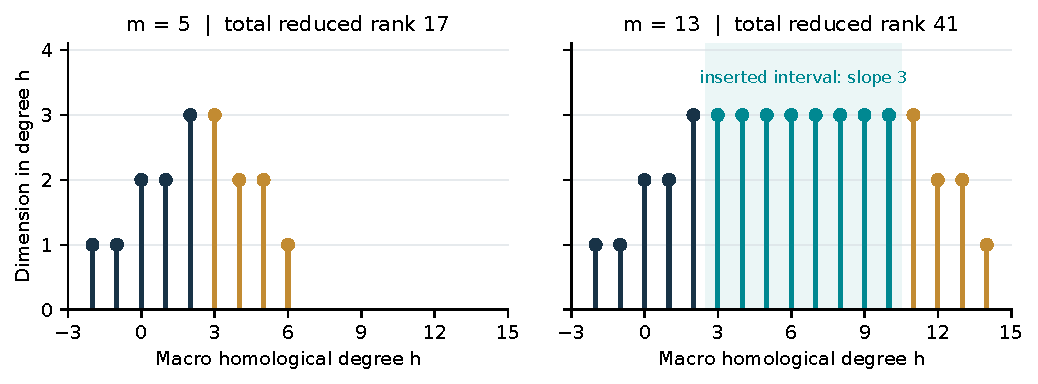
\includegraphics[width=\linewidth]{figures/exact_profile.pdf}
\caption{Exact reduced homological profiles of
\(\sigma_1^m\sigma_2^{-1}\sigma_1\sigma_2^{-1}\).
The dark lower region is fixed, the gold upper region translates by
\(m-5\), and the teal interval contributes rank \(3\) in each inserted
degree. Both panels are generated from exact output; the recurrence is
proved independently of the plotted examples.}
\label{fig:profile}
\end{figure}

\subsection{Paired long-run homology measurements}

The recurrence benchmark uses seven A/B/A rounds per case, a separate
seven-pair A/A control, and fresh computation caches. A is the ordinary
macro backend; B is the exact recurrence. A returns an explicit degree
dictionary and B an exact compressed profile. Their complete homological
information agrees. Expansion of B's compact interval is excluded from
its timed task, because compact output is the interface whose complexity
is being measured.

The benchmark contains three families at selected lengths
\(17,65,257,1025\), plus a below-threshold no-compression control.
There is no braid simplification or earlier recognition filter in these
timings. The three largest-length results are:

\begin{center}
\small
\begin{tabular}{lrrrrr}
\toprule
Family, \(m=1025\) & \(\N(m)\) & \(\N_0\) &
A (ms) & B (ms) & Paired A/B\\
\midrule
Two strands & 1,027 & 4 & 3.639 & 0.084 & 39.42\\
Figure-eight context & 15,393 & 93 & 44.000 & 0.637 & 69.12\\
Mixed four-strand link & 18,486 & 126 & 37.998 & 0.931 & 44.05\\
\bottomrule
\end{tabular}
\end{center}

Durations are medians, with A averaged over the two surrounding calls in
each round. The final column is the median of the paired round ratios,
not the quotient of the separately displayed medians.
The mixed four-strand input is
\(\sigma_1^m\sigma_2^{-1}\sigma_3\sigma_2^{-1}\);
its measured odd-\(m\) closure is a link, and the benchmark computes its
marked reduced homology.

The no-compression control had median A/B \(1.021\), with individual
ratios from \(0.723\) to \(1.355\). The separate A/A control had median
second/first \(1.064\). Small durations are visibly noisy.
The algebraic count reduction, the exact equality checks, and the
asymptotic theorem are stronger evidence than a single microbenchmark
ratio. These are standalone full-homology gains. By
\cref{cor:dominant}, the knot families in the proved long-run range are
already structurally decided by the baseline.

\begin{figure}[htbp]
\centering
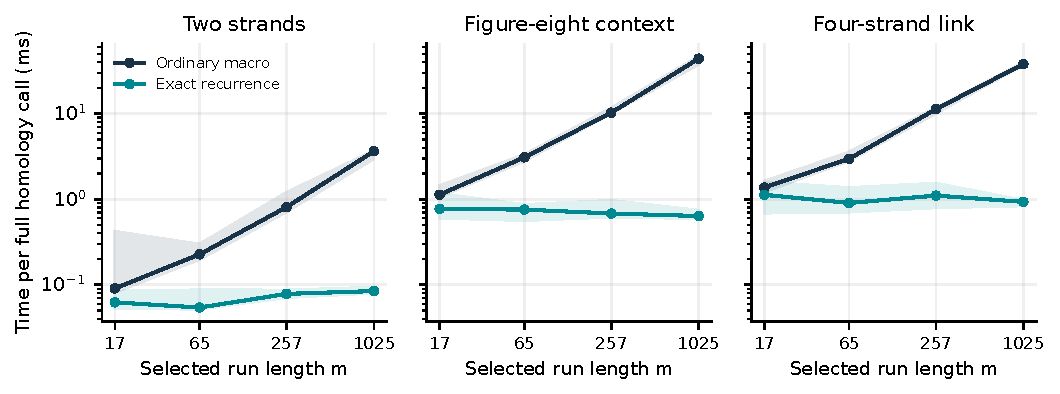
\includegraphics[width=\linewidth]{figures/tail_scaling.pdf}
\caption{Median standalone homology times at four run lengths.
Shading shows the interquartile ranges of the retained paired samples.
Both axes are logarithmic. The finite reference is unchanged within each
family; the measurements still show ordinary host and timing variability.}
\label{fig:tailtimes}
\end{figure}

\subsection{Streaming: memory savings with an observed time cost}

The streaming experiment uses eight cases and seven randomized rounds,
with five fresh calls per arm per round. Each round includes an
identical original-backend control. Full ranks, homological profiles,
chain dimensions, and boundary ranks are compared. Differential-square
checking occurs before timing. Memory tracing occurs in separate fresh
runs, so its instrumentation does not contaminate the duration
measurements.

Across these cases, the paired original/streamed time ratios range from
\(0.265\) to \(0.698\): complete streamed homology is slower.
The original/streamed peak traced-allocation ratios range from
\(1.028\) to \(3.064\): peak allocation is smaller.
A/A time ratios range from \(0.849\) to \(1.198\).
The allocation measurements are newly traced Python allocations from
\code{tracemalloc}, not process RSS or a hardware memory lower bound.

\begin{figure}[htbp]
\centering
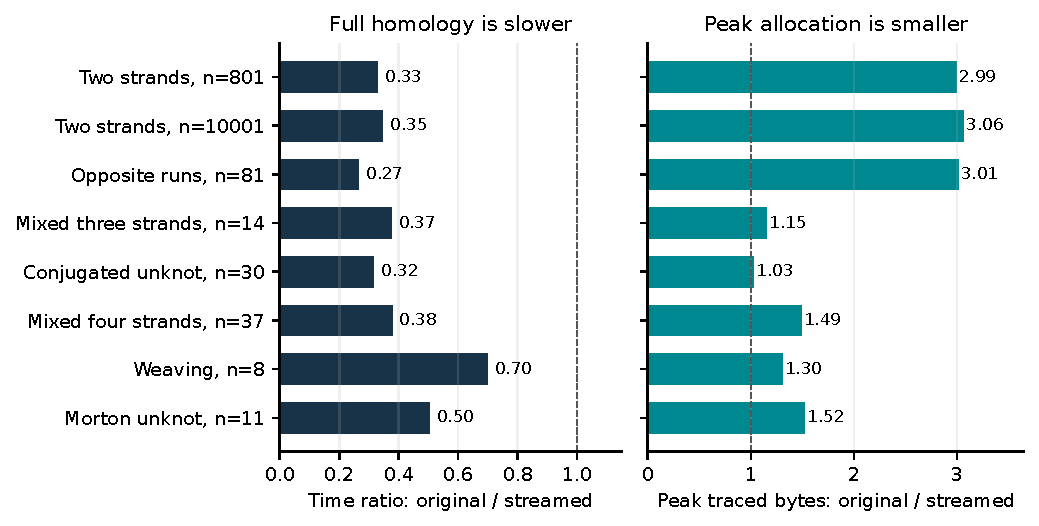
\includegraphics[width=\linewidth]{figures/streaming_tradeoff.pdf}
\caption{The full-homology time--space tradeoff across all eight streamed
benchmark cases. A ratio below one on the left means the streamed
implementation is slower. A ratio above one on the right means it uses
fewer peak traced bytes. The dashed line is equality.}
\label{fig:streamtradeoff}
\end{figure}

The repository's actual Morton input is an informative complete
unknot example:
\[
[-3,-3,2,-3,2,1,1,1,-2,1,-2]\quad(b=4).
\]
It has 768 macro states and 2,799 reduced basis elements.
In degrees \(-5,\ldots,6\), its chain dimensions and outgoing ranks are
\[
\begin{array}{r|rrrrrrrrrrrr}
h&-5&-4&-3&-2&-1&0&1&2&3&4&5&6\\ \hline
d_h&8&48&138&270&417&518&510&414&278&142&48&8\\
r_h&8&40&98&172&245&272&238&176&102&40&8&0
\end{array}
\]
so \eqref{eq:betti} gives one class in degree zero and no others.
The streamed run retains at most 308 state entries and 272 pivots.
The dense full-matrix sum is \(Q=1{,}009{,}952\) bits; the ordinary
streamed live envelope is 140,760 bits.
These are two structural bounds, not measured byte values.

The measured Morton medians are 27.360 ms for the original and
50.385 ms for streaming. Peak traced allocations are 1,441,224 and
946,172 bytes, respectively, a \(1.523\)-fold reduction.
Thus the implementation improves memory use on an actual full-rank-one
calculation but does not justify replacing the faster default on
time grounds.

For \(\sigma_1^{10001}\), full original and streamed computations take
37.742 and 100.604 ms, while streamed early recognition takes 0.118 ms
and visits four states. The four-strand mixed case of 37 crossings
visits 192 of 2,048 states before an early lower bound exceeds one.
These demonstrate the correctness and possible value of an early
backend endpoint. They do not measure its value after the existing
structural and modular filters.

\subsection{Separating encoding savings from recognition savings}

The structural experiment uses
\[
\gamma_m=\sigma_1^m\sigma_2^{-(2m-1)}\sigma_3^m,\qquad
b=4,\quad m\ge3\text{ odd}.
\]
These are one-component homogeneous braids with exponent sum \(1\),
zero Rasmussen interval, and positive canonical genus.
The homogeneous-genus criterion already proves nontriviality.
The coarse exponent-sum obstruction alone does not do so.

One experiment times a direct RLE certificate against expansion of
the word, checked PD construction, and the existing Seifert certificate.
A second uses fresh prebuilt diagrams and changes only the opt-in
\code{use_braid_profile} argument to the recognizer; construction is
outside that second timer.

\begin{center}
\small
\begin{tabular}{rrrrr}
\toprule
\(m\) & Crossings & Expanded construction / RLE &
Profile off / on & Pipeline A/A\\
\midrule
17 & 67 & 107.71 & 2.76 & 0.964\\
129 & 515 & 999.73 & 4.49 & 1.168\\
1025 & 4099 & 6645.13 & 4.03 & 1.039\\
4097 & 16387 & 36063.64 & 3.48 & 0.884\\
\bottomrule
\end{tabular}
\end{center}

All ratios are medians of paired rounds. The large construction-inclusive
ratios measure the explicit encoding difference: three integer runs
versus thousands of crossings and PD incidences. They are not general
recognition speedups. The prebuilt-diagram experiment shows an additional
constant-factor improvement on these selected structural cases.
All decisions and all compared Seifert metadata agree.
The Morton structural-only control remains \code{INCONCLUSIVE} in
both implementations; its full recognizer is excluded from that
experiment.

The first shorter batches showed substantial timer noise. Both pilot
files are retained, and the final script uses fixed size-based larger
batches rather than selecting favorable samples.
The reported A/A controls still require approximate interpretation.
The polynomial encoded-input theorem is independent of those timings.

\section{What still obstructs a general quasi-polynomial bound}\label{sec:barriers}

\subsection{Finite matching types do not bound multiplicity}

The macro state space separates geometry from algebraic copies.
Even a very small collection of boundary matchings can occur with
exponentially large multiplicities. Streaming changes how those copies
are visited; it does not eliminate the copies. The one-run recurrence
does eliminate a repeated algebraic region, but only after a fixed
finite context has been solved.

The three-strand obstruction in Kelom\"aki--Sch\"utz~\cite{ks26}
is particularly decisive against a universal width-only argument.
Some constant-strand families have exponentially growing total Betti
number, so any algorithm explicitly retaining a basis must expand
exponentially. Their specialized polynomial computation shows why this
is a representation obstruction rather than an impossibility theorem
for compact output.
The same lesson applies to scalar transfer matrices: their coefficients
can encode very large counts, but a transfer formula for the Euler
characteristic does not automatically determine homology ranks.

Likewise, the restriction \(t=O(\log n)\) in
\eqref{eq:prior-bound} is substantive. It cannot be removed by calling
the supplied run count a width parameter. A general diagram may have
\(t=\Theta(n)\), and the existence of some small topological
decomposition does not imply a polynomial procedure to find it with
short, verifiable moves.

\subsection{Why several long variables need more than interpolation}

A plausible next direction is to allow several large exponents at
once. Even the simplest example rules out one overly strong formulation.

\begin{proposition}[No single eventual polynomial in all twist lengths]
\label{prop:chambers}
There is no polynomial \(p(m,\ell)\) agreeing, for all sufficiently
large \(m,\ell\) with \(m-\ell\) odd, with the total reduced
characteristic-two Khovanov rank of the closed braid
\(\sigma_1^m\sigma_1^{-\ell}\).
\end{proposition}

\begin{proof}
The braid cancels to \(\sigma_1^{m-\ell}\), a two-strand torus knot
when \(m-\ell\) is odd. Its reduced rank is \(|m-\ell|\).
This last fact also follows directly from the one-run normal form:
there is one class in degree zero, none in degree of magnitude one,
and one in each subsequent degree through magnitude \(|m-\ell|\).

If \(p\) existed, fix any sufficiently large integer \(\ell\).
For infinitely many admissible \(m>\ell\),
\(p(m,\ell)=m-\ell\). A one-variable polynomial with infinitely many
zeros is zero, so \(p(x,\ell)=x-\ell\) identically in \(x\).
This holds for infinitely many \(\ell\), hence
\(p(x,y)=x-y\) as a two-variable polynomial.
It contradicts the required value \(\ell-m\) for admissible
\(\ell>m\).
\end{proof}

The cancellation in this example is cheap and should be performed first
in a practical recognizer. Its role is conceptual: comparable exponents
can produce different asymptotic chambers separated by equalities of
lengths. A multivariable theorem might use piecewise polynomial,
quasi-polynomial, or rational generating descriptions with explicit
chamber conditions. A few numerical values cannot select the correct
description or prove its validity throughout a large orthant.

\subsection{A sufficient representation target}

The useful target is a compact algebraic model closed under the operations
the algorithm actually performs. For a tangle fragment it must include
boundary data, grading shifts, multiplicities, differentials, and the
maps used in subsequent gluing. A list of dimensions is insufficient.

\Needspace{14\baselineskip}
\begin{proposition}[Conditional complexity contract]\label{prop:contract}
Suppose every \(n\)-crossing input admits a constructible decomposition
with \(\poly(n)\) composition steps. Assume:
\begin{enumerate}
\item each intermediate fragment has a faithful algebraic description
of at most \(S(n)\) bits, including all multiplicities and map data;
\item each composition, reduction, and final rank-one decision can be
performed in \(\poly(n,S(n))\) bit operations while preserving a
description of that size;
\item the construction and the correctness of every representation
change have the same total complexity bound.
\end{enumerate}
If \(S(n)=2^{O((\log n)^2)}\), this gives a complete
\(n^{O(\log n)}\)-time recognition algorithm.
\end{proposition}

\begin{proof}
There are polynomially many steps, each of polynomial degree independent
of \(n\) in \(n\) and \(S(n)\). Their sum, including the construction and
final decision, remains \(2^{O((\log n)^2)}\).
Faithfulness makes the final rank-one decision equivalent to
\eqref{eq:detector}.
\end{proof}

This proposition is a contract for future theorems, not a proof that such
descriptions exist. In particular the first assumption forbids hiding
large basis multiplicity inside a supposedly small number of geometric
types, and the second forbids an implicit exponential expansion during
composition. The third distinguishes finding a useful decomposition
from merely asserting its existence.

The present recurrence satisfies this kind of contract for one finite
context followed by a homogeneous repeated chain region. It gives a
concrete example of how much information can be compressed while still
recovering exact ranks. Extending that closure property to interacting
regions is the central algebraic problem.

\section{Further research questions and proposed work programme}
\label{sec:research}

The following topics are ordered by their connection to the actual
remaining bottlenecks. Each has a concrete mathematical or experimental
completion criterion. They are proposals, not claimed consequences of
the current implementation.

\subsection{Reduce the effective context amplitude}

\begin{question}\label{q:amplitude}
Can the raw crossing span \(W\) be replaced by the degree span of a
smaller context model that retains both dot actions and the distinguished
saddle?
\end{question}

The proof of \cref{thm:recurrence} uses a common support interval for the
\(I\) and \(E\) context sectors and compatibility with their maps.
Suppose an explicitly constructed equivalence of this two-sector
context has degree-preserving forward and backward maps, with contracting
homotopies, all compatible with both exterior dot actions and the
distinguished saddle. If both resulting sector complexes are supported
in \([a',c']\), the same proof gives threshold \(c'-a'+2\).
Compatibility is required at the level of maps and homotopies.
An ordinary homotopy equivalence of the underlying complexes alone
does not suffice; transporting operators through an arbitrary
contraction can introduce additional terms.

A first implementation should perform local contractions in the open
tangle category and transport the saddle, dot actions, and contracting
homotopies. It should output an equivalence witness and measure both
the reduced amplitude and the resulting matrix size.
A useful negative outcome would be a family where amplitude is small
but the equivariant context dimension still grows exponentially.
That would isolate the next barrier more accurately than crossing
count alone.

\subsection{Two interacting variable regions before arbitrary many}

\begin{question}\label{q:two}
For two distinguished runs, can their simultaneous long region be
described by finitely many exact face and chamber models whose evaluation
is polynomial in the two exponent bit lengths?
\end{question}

The one-run interior is controlled by \(D_E+L\). With two selected
turnbacks, there are two commuting local dot sums and several
\(I/E\) sectors. The total homological degree combines both local
coordinates, so the number of copies along a diagonal changes near
the boundary of the exponent rectangle. A faithful model must retain
those incidences, not simply add two independently computed slopes.

Begin with adjacent and nonadjacent generators, both relative signs,
all original component parities, and the cancellation family in
\cref{prop:chambers}. Require an exact symbolic formula whose chamber
conditions are proved, then compare complete small profiles with the
crossing cube. Only after the two-variable case is understood should
one study an \(s\)-variable face system with up to \(2^s\) sectors.
Even that sector count would not bound internal module complexity.

\subsection{Restore quantum information}

\begin{question}\label{q:quantum}
What is the exact bigraded refinement of the one-reference recurrence,
including the shifts of both boundary regions and the repeated interval?
\end{question}

The ungraded deformation \(D_E+L\) combines maps with different original
bidegrees. The slope identity gives total dimension and does not place
the smoothing's original bigraded groups in the long complex.
A correct refinement must carry the quantum shifts in the integer-twist
normal form before flattening the central groups.
One possible output is a rational generating expression in homological
and quantum variables, with finite boundary corrections. Its validity
and output size have to be proved.
The completion criterion is agreement with an independently bigraded
cube on both signs and mixed contexts, not just recovery of the Jones
Euler polynomial.

\subsection{Odd characteristics and integral torsion}

\begin{question}\label{q:integral}
Can a signed periodic central model replace \(F\) over fields of odd
characteristic and over the integers?
\end{question}

The current square-zero calculation and weight cancellation use
characteristic two. Over the integers, twist differentials alternate
dot sums and differences; signs also interact with tensor degrees.
A period-two central model is a natural object to examine, but using
the present \(D_E+L\) unchanged is invalid.
An integral algorithm additionally needs Smith-form or module data,
with the bit lengths of torsion invariants included in its complexity.
The first result should be a fully signed local and contextual theorem,
followed by a recurrence for isomorphism types or a precisely weaker
rank statement.

\subsection{Decision certificates smaller than full homology}

\begin{question}\label{q:certificate}
Can a rank-greater-than-one witness be represented and verified compactly
on inputs that evade the structural and modular filters?
\end{question}

There is a concrete algebraic witness to seek. In a chain complex with
total differential \(d\), find two cycles \(z_1,z_2\) and two linear
functionals \(\ell_1,\ell_2\) satisfying
\[
dz_j=0,\qquad \ell_i d=0,\qquad \ell_i(z_j)=\delta_{ij}.
\]
Then the two homology classes are independent: any boundary relation
between them is annihilated by both functionals. This elementary
criterion gives a verifiable target.
An explicit witness can be exponentially long, so the research problem
is a representation that supports these products without expansion.
The streamed lower bound already proves a decision but does not yet
produce such a portable compressed cycle--cocycle witness.

Unknot certificates need a different positive mechanism, such as a
small contraction to the one-generator reduced complex or a
topological simplification certificate. A method that quickly produces
two surviving classes on many knots still needs a complete, costed
endpoint on hard unknots.

\subsection{Use tangle invariants with explicit algebraic size accounting}

\begin{question}\label{q:curves}
Can immersed-curve or related four-ended tangle descriptions support
exact repeated gluing with compact multiplicities and controlled local
systems?
\end{question}

The framework of Kotelskiy--Watson--Zibrowius is a serious source of
structure~\cite{kwz}. The relevant complexity parameters would include
curve segments, intersections under twisting, local-system ranks and
entries, and the cost of cancelling the resulting Floer-type complex.
A picture with few curves may still encode many intersections or a
large local system. The first milestone should translate one delivered
long-run example into that representation and recover its threshold,
slope, and boundary corrections with explicit cost accounting.

\subsection{Recover speed while preserving the streamed memory bound}

\begin{question}\label{q:streamspeed}
Which bounded low-level changes recover the streamed backend's observed
time loss without restoring unbounded tables?
\end{question}

Candidates include a compiled exact bitset kernel, small-label tables
admitted only under an explicit slot cap, reused neighboring state keys,
and a more efficient geometry construction.
The benchmark currently shows a real time cost, so a default switch
would be premature.
Any follow-up should report complete output equality, paired A/B and
A/A timings, total versus live state counts, map-compilation counts,
and separate traced-allocation measurements on the same inputs.

A related question is whether the sweep should start at the other
homological end. Reversing the sweep requires the correct transposed
local maps and grading conversion. A preflight estimate may choose an
end, but an estimate of where homology is likely cannot substitute
for the exact incident ranks required by an early decision.

\subsection{Benchmark the unresolved part of the pipeline}

\begin{question}\label{q:corpus}
Which checked inputs actually reach the expensive endpoint after all
current inexpensive certificates, and what algebraic feature predicts
their cost?
\end{question}

Record the exit stage of every case, rather than timing all backends
on examples already decided at the front. Include actual hard unknot
fixtures, determinant-one nontrivial knots, mixed-sign braids of at
least four strands, and examples with large intermediate but small
final homology. Retain source provenance and the distinction between
PD-only and braid-source inputs.
The correct metrics include crossings, runs, degree span, maximum
layer dimension, cancellation fill, map recompilation, and the
compressed context size from \cref{q:amplitude}.
Artificially labeling an easy torus or three-strand example as hard
would make this research programme less informative.

\subsection{Cost the hierarchy route operation by operation}

\begin{question}\label{q:hierarchy}
Can the remaining hierarchy steps be given explicit input/output bit
contracts and composed into a complete quasi-polynomial runtime proof?
\end{question}

The required ledger includes hierarchy length, boundary-pattern size,
surface-coordinate bit length, component tracking after cutting,
product-region recognition, and the search cost of each next surface.
Polynomial certificate verification must be kept separate from finding
the certificate. Compact normal coordinates must remain compact through
every update.
Lackenby's current results provide substantial ingredients
\cite{lackenby26}; completing this ledger would be an independent route,
not a corollary of the present Khovanov recurrence.

\subsection{Formalize the finite algebraic core first}

\begin{question}\label{q:formal}
Which parts admit a small proof-assistant development with a stable
boundary to the topological literature?
\end{question}

The square-zero calculation, signed interval bookkeeping, rank identity,
positive and negative profile formulas, and cycle--cocycle witness
criterion are finite algebra and arithmetic. They are natural first
targets. A formalization should expose the local tangle-normal-form
assumption and then separately formalize or import its topological
proof. A machine-checked recurrence conditional on that assumption is
valuable, but is not a formalization of the complete unknot detector.
The current package contains conventional proofs and executable
cross-checks, not a Lean proof.

\subsection{A proposed sequence of research milestones}

\begin{enumerate}
\item Integrate the additive code and preserve the default dispatcher.
Reproduce the 254-method suite and the independent cube checks.
\item Build dot- and saddle-compatible context contractions and measure
effective amplitude on filter-undecided examples.
\item Prove a complete two-variable theorem, including its chambers,
component parities, and compact output.
\item Construct and independently verify compact nontriviality witnesses,
with an explicit positive endpoint for unknot cases.
\item Test a representation closed under repeated tangle gluing against
the size and operation contract in \cref{prop:contract}.
\item Pursue the hierarchy cost ledger in parallel, so the programme
does not depend on one algebraic representation succeeding universally.
\end{enumerate}

The immediate work is concrete and testable. A general quasi-polynomial
claim should be made only when both a compact representation and the
cost of every operation on it have been proved, including construction
and the final decision.

\section{Integration, reproducibility, and provenance}\label{sec:integration}

\subsection{Package layout and proposed repository placement}

The archive contains the complete modified \code{fast/} tree and an
untouched \code{reference/fast/} snapshot from the pinned revision.
The integration patch is relative to
\code{Topology/UnknotRecognition/fast}. It adds the modules and tests
described below and the optional source-profile argument; it does not
alter the default recognition dispatch.
The article and research artifacts can be placed in a new report
directory under \code{Topology/UnknotRecognition/reports/}, using the
next free report number at integration time.

\begin{center}
\small
\begin{tabular}{p{0.43\linewidth}p{0.48\linewidth}}
\toprule
File or directory & Purpose\\
\midrule
\code{article/main.tex} and section files &
Complete article source, with an ordinary LaTeX bibliography.\\
\code{article/main.pdf} & Compiled and visually checked article.\\
\code{article/figures/} & Vector figures and PNG previews, generated
from exact output or retained measurements.\\
\code{fast/fastunknot/twist/tail.py} &
Exact one-reference homological recurrence and compact-profile API.\\
\code{fast/fastunknot/twist/streaming.py} &
Bounded-cache, degree-streamed full homology and early recognition.\\
\code{fast/fastunknot/braid_profile.py} &
Run-encoded structural certificates and the dominated signature
experiment.\\
\code{fast/fastunknot/twist/continuation.py} &
Raw RLE command-line and Python frontend.\\
\code{fast/tests/} & All inherited and new regression tests.\\
\code{tools/} & Portable audits, benchmarks, figure regeneration,
validation, and article build scripts.\\
\code{results/} & Raw measurements, pilot runs, exact comparison
records, and the complete test log.\\
\code{reference/} & Pinned baseline and detailed proof/accounting
audit notes.\\
\code{integration.patch} & Additive patch for review against the
pinned baseline.\\
\bottomrule
\end{tabular}
\end{center}

The baseline MIT No Attribution (MIT-0) license is retained.
No remote repository write or
default-backend replacement is part of this deliverable.
The accompanying integration guide gives the exact paths and patch
check command.

\subsection{Interfaces and examples}

From the package's \code{fast/} directory, the new frontend accepts
run-encoded JSON:
\begin{lstlisting}
{"strands": 3, "runs": [[1, 1001], [2, -1], [1, 1], [2, -1]]}
\end{lstlisting}
The corresponding commands are:
\begin{lstlisting}
python -m fastunknot.twist.continuation input.json
python -m fastunknot.twist.continuation input.json \
  --mode homology --method tail --check-d2
python -m fastunknot.twist.continuation input.json \
  --mode homology --method streaming
python -m fastunknot.twist.continuation input.json --mode profile
\end{lstlisting}

The default is recognition with the tail method selected for any
necessary exact endpoint. Recognition first checks the original
one-component closure and tries the direct structural certificate.
Only an inconclusive certificate reaches the selected backend.
Full homology mode always computes the selected full exact homology,
including for links; it does not stop after a cheap knot verdict.
Profile mode returns only the structural certificate.
The methods \code{tail}, \code{streaming}, and \code{macro} are explicit
choices.

A Python call avoids JSON serialization limits for extremely large
integers:
\begin{lstlisting}
from fastunknot.twist.core import Run
from fastunknot.twist.tail import tail_homology, profile_dimension

m = (1 << 100000) + 1
answer = tail_homology(2, [Run(1, m)], check_d2=True)
assert answer["reduced_rank"] == m
assert answer["reference"]["stats"]["basis"] == 4
assert profile_dimension(answer["degree_profile"], m) == 1
\end{lstlisting}

The standard Python JSON integer conversion has a decimal-digit
limit in this runtime. The API supports the tested 100,001-bit
integers directly; the CLI does not disable that general runtime
limit. JSON also converts dictionary degree keys to strings.
The documentation identifies the schema and inclusive interval
semantics so downstream consumers do not confuse a large encoded
endpoint with an explicit array index range.

Existing checked diagrams can opt into the source specialization via
\code{recognize(diagram, use_braid_profile=True)} or the production
\code{--braid-profile} option. It is used only with retained checked
braid source. A PD-only diagram does not acquire invented braid
provenance, and a later diagram factor is not assumed to share the
original source braid.

\Needspace{15\baselineskip}
\subsection{Reproduction commands}

From the archive root:
\begin{lstlisting}
PYTHONPATH=fast python -m unittest discover -s fast/tests -v
python tools/audit_long_twist.py
python tools/audit_slope.py
python tools/benchmark_tail.py
python tools/benchmark_streaming.py --rounds 7 --batch 5
python tools/benchmark_braid_profile.py --rounds 7
python tools/make_figures.py
bash tools/build_article.sh
\end{lstlisting}

The exact outputs originally used in the article are retained.
Rerunning measurements overwrites their default target files; retain a
copy or specify a separate output path for comparison.
Wall-clock measurements on another machine are expected to differ.
The scripts use package-relative imports, fixed stated random seeds,
and standard-library exact arithmetic for the core algorithms.
Matplotlib is used only to regenerate plots.
Building the article requires a conventional LaTeX installation with
the packages named in the preamble and \code{latexmk}.

The independent recurrence audit was executed successfully before
being relocated into the final package. The relocated script changes
paths and explanatory text, not the tested algebra, and its raw result
file is retained unchanged. Its provenance note states this explicitly.
The final integrated 254-method suite was run on the delivered combined
implementation.

\subsection{Evidence boundaries and integration decisions}

The proofs establish a theorem for finite complexes obtained from the
stated local normal form. The implementation comparisons check that
the delivered code computes that model on the tested inputs.
Neither is a proof-assistant formalization of the entire topology
dependency chain.
Benchmarks establish observations on specified input families and
execution conditions; they do not establish a distribution-free
performance claim.

For integration, the evidence supports adding the tested APIs, research
documentation, and opt-in source-profile stage. The streamed backend
should remain selectable on memory grounds while its measured time
loss is addressed. A future automatic dispatcher should be justified
on the subset of inputs reaching the expensive endpoint, with both
time and memory objectives stated.

The main unresolved theorem is universal closure of a compact
representation under construction, gluing, reduction, and exact
decision. The finite-threshold result supplies one such closure
mechanism in a controlled setting, together with enough source,
proof, and experimental detail to make the next stage of research
reviewable and reproducible.

\begin{thebibliography}{99}
\addcontentsline{toc}{section}{References}
\raggedright

\bibitem{repo}
Vladimir Reshetnikov, \emph{ProveIt: Topology/UnknotRecognition}.
Repository revision
\code{ea2abcb115aaa58f0b193ce1e045c2def983e1e6},
retrieved 8 October 2026. In particular, reports 10--12,
\code{synthesis/twist.tex}, \code{synthesis/research_updates.tex},
and the complete \code{fast/} source and tests.
\url{https://github.com/VladimirReshetnikov/ProveIt/tree/ea2abcb115aaa58f0b193ce1e045c2def983e1e6/Topology/UnknotRecognition}.

\bibitem{bn05}
Dror Bar--Natan, \emph{Khovanov's homology for tangles and cobordisms}.
Geometry \& Topology \textbf{9} (2005), 1443--1499.
\url{https://arxiv.org/abs/math/0410495v2}.
\url{https://doi.org/10.2140/gt.2005.9.1443}.

\bibitem{bn07}
Dror Bar--Natan, \emph{Fast Khovanov homology computations}.
Journal of Knot Theory and Its Ramifications \textbf{16} (2007),
243--255.
\url{https://arxiv.org/abs/math/0606318}.

\bibitem{thompson}
Benjamin Thompson, \emph{Khovanov complexes of rational tangles}.
arXiv:1701.07525v2, revised 12 December 2018.
In particular, Proposition 4.1.
\url{https://arxiv.org/abs/1701.07525v2}.

\bibitem{jaeger}
Thomas C. Jaeger, \emph{A remark on Roberts' totally twisted Khovanov
homology}. arXiv:1109.1805 (2011).
In particular, Theorem 3.1 and its local change-of-basis proof.
\url{https://arxiv.org/abs/1109.1805}.

\bibitem{kwz}
Artem Kotelskiy, Liam Watson, and Claudius Zibrowius,
\emph{Immersed curves in Khovanov homology}.
arXiv:1910.14584v2, revised 17 December 2019.
\url{https://arxiv.org/abs/1910.14584v2}.

\bibitem{km}
Peter B. Kronheimer and Tomasz S. Mrowka,
\emph{Khovanov homology is an unknot-detector}.
Publications Math\'ematiques de l'IH\'ES \textbf{113} (2011), 97--208.
\url{https://arxiv.org/abs/1005.4346}.

\bibitem{ks26}
Tuomas Kelom\"aki and Dirk Sch\"utz,
\emph{On computational complexity of Khovanov homology}.
arXiv:2601.02119v1, 5 January 2026.
In particular, Theorems 1.2 and 1.3.
\url{https://arxiv.org/abs/2601.02119v1}.

\bibitem{lobb}
Andrew Lobb, \emph{Computable bounds for Rasmussen's concordance
invariant}. Compositio Mathematica \textbf{147} (2011), 661--668.
In particular, Theorem 1.10.
\url{https://arxiv.org/abs/0908.2745v2}.
\url{https://doi.org/10.1112/S0010437X10005117}.

\bibitem{abe}
Tetsuya Abe, \emph{The Rasmussen invariant of a homogeneous knot}.
Proceedings of the American Mathematical Society \textbf{139} (2011),
2647--2656. In particular, Theorems 2.3 and 3.4.
\url{https://arxiv.org/abs/1003.5392}.

\bibitem{cromwell}
Peter R. Cromwell, \emph{Homogeneous links}.
Journal of the London Mathematical Society (2) \textbf{39} (1989),
535--552.
\url{https://doi.org/10.1112/jlms/s2-39.3.535}.

\bibitem{feller}
Peter Feller, \emph{The signature of positive braids is linearly
bounded by their first Betti number}.
arXiv:1311.1242v2, revised 18 July 2015.
In particular, Section 4.
\url{https://arxiv.org/abs/1311.1242v2}.

\bibitem{lackenby26}
Marc Lackenby, \emph{Incompressible surfaces, hierarchies and unknot
recognition}. arXiv:2607.23350v1 (July 2026).
In particular, Section 9 and Proposition 9.1; the compressed-surface
and verification results should be read with their individual
hypotheses and cost parameters.
\url{https://arxiv.org/abs/2607.23350v1}.

\bibitem{openaimath}
OpenAI, \emph{Mathematical manuscripts and supporting proof artifacts}.
Repository README and manuscript catalogue, inspected 8 October 2026.
README blob \code{8ac0cb7dbf1f38ad3b7480310d4e1d9482f0cfe8}.
No theorem from this collection is assumed in the present proofs.
\url{https://github.com/openai/math}.

\end{thebibliography}

\end{document}
